\documentclass[a4paper,11pt]{article}

\usepackage[utf8]{inputenc}

\usepackage{graphicx}
\usepackage{caption}
\usepackage{subcaption}

\usepackage{pgfplots}
\pgfplotsset{compat=1.18} 

\usepackage{minted}

\begin{document}

\title{
    \textbf{Assignment 3 Report - Sorted array search in Java}
}
\author{Dean Tsankov}
\date{\today}

\maketitle

\section*{Introduction}
Searching for an item in an unsorted array is quite time expensive. If there is no order to the elements, the only way to find a specific one is to go through the whole data structure. This report will present how things will become much easier and potentially more time efficient if the array is sorted.

\section*{Base Case}

Let us get an idea of what a benchmark on the standard case of traversing an unsorted array to find an element, looks like. Using the provided method {\tt unsorted\textunderscore search()} and plugging it into a benchmark code very reminiscent of the one in the first assignment, we can conclude a few things. A plot of the benchmark could also help us get an understanding.

\begin{figure}[H]
    \centering
    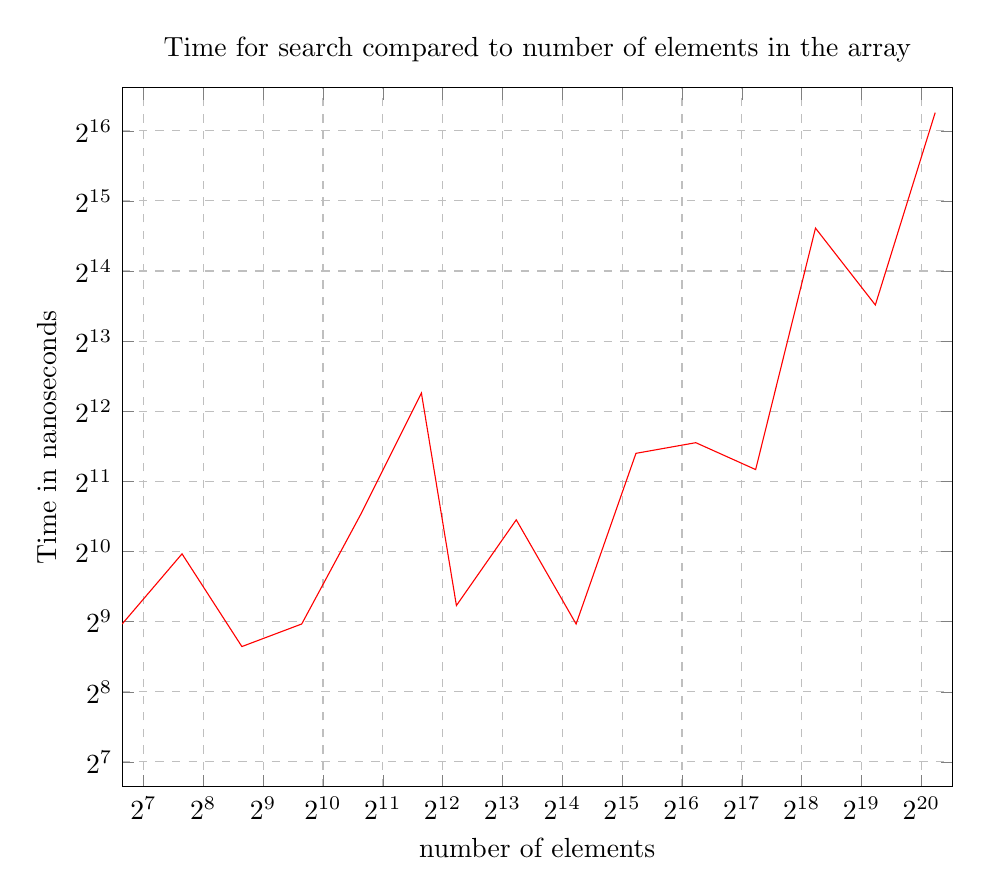
\begin{tikzpicture}
        \begin{axis}[
            title={Time for search compared to number of elements in the array},
            width=\linewidth,
            xlabel={number of elements},
            ylabel={Time in nanoseconds},
            xmode=log,
            log basis x={2},
            ymode=log,
            log basis y={2},
            xmin=100, xmax=1500000,
            ymin=100, ymax=100000,
            ymajorgrids=true,
            xmajorgrids=true,
            grid style=dashed,
        ]
        
        \addplot[
            color=red,
            ]
            coordinates {
            (100,500)(200,1000)(400,400)(800,500)(1600,1500)(3200,4900)(4800,600)(9600,1400)(19200,500)(38400,2700)(76800,3000)(153600,2300)(307200,25000)(614400,11700)(1228800,78300)
            };
            
            
        \end{axis}
        \end{tikzpicture}
    \caption{Over unsorted array(samples are average of 3 measurements)}
    \label{fig:plot1}
\end{figure}

As we might expect the points are a bit sporadic due to the unordered nature of the array. Due to this I decided to take the average time for each array size test of three different executions of the search algorithm. This gives a slightly more general appearance to the plot and allows us to still see a somewhat linear increase in the time. We get this from the fact that the graph axes are mapped logarithmically.

In this case our last sample is the time over an array with 1228800 and the measured time is {\tt 78300ns}.

\section*{Sorted Array}
We now try to benchmark the code using the given snippet for generating an already sorted array of elements. As well as implementing the single optimisation step of stopping our search if the current element is already larger than the one we are searching for. Here is the search method:


\begin{minted}[
frame=single,
framesep=2mm,
baselinestretch=1.2,
fontsize=\footnotesize,
]{java}
    (...)
     public static boolean sorted_search(int[] array, int key) {
        for (int index = 0; index < array.length; index++) {
            if (array[index] == key) {
                return true;
            }
            if(array[index] > key){
                return false;
            }
        }
        return false;
    }
    (...)
\end{minted}    

Here I present the new samples over the sorted array: 

\begin{figure}[H]
    \centering
    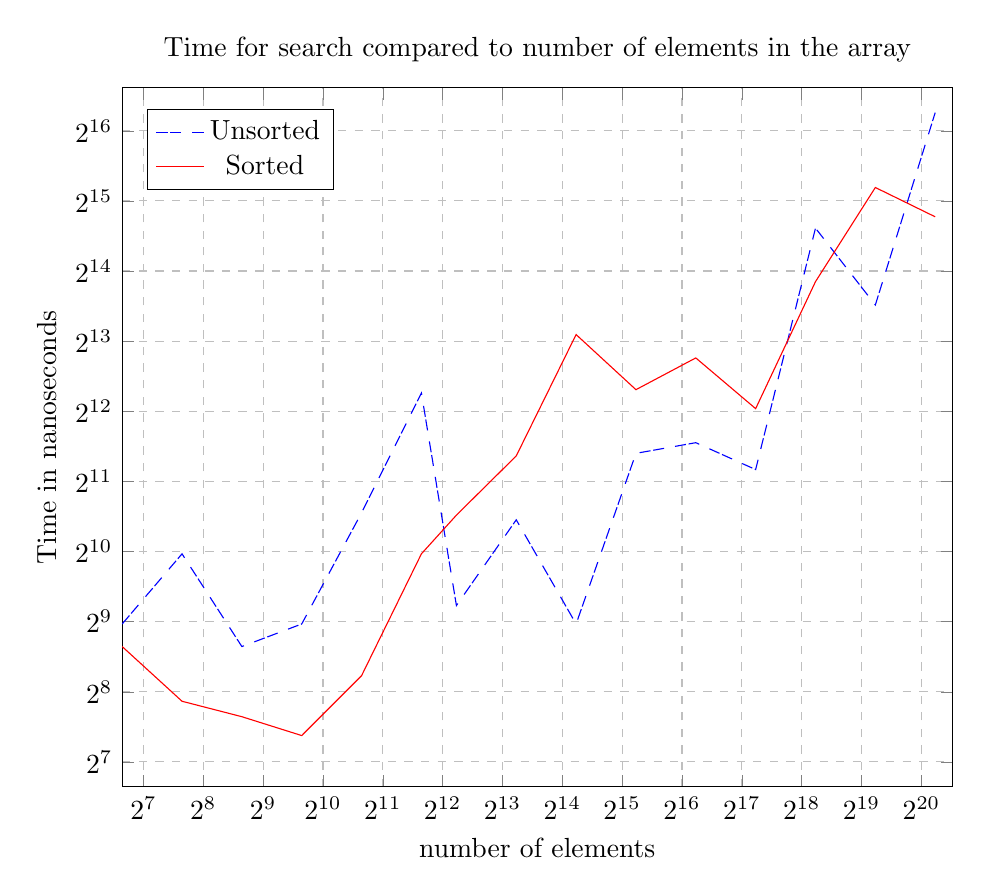
\begin{tikzpicture}
        \begin{axis}[
            title={Time for search compared to number of elements in the array},
            width=\linewidth,
            xlabel={number of elements},
            ylabel={Time in nanoseconds},
            xmode=log,
            log basis x={2},
            ymode=log,
            log basis y={2},
            xmin=100, xmax=1500000,
            ymin=100, ymax=100000,
            ymajorgrids=true,
            xmajorgrids=true,
            grid style=dashed,
            legend pos=north west,
        ]
        
        \addplot[
            color=blue,
            dash pattern=on 4pt off 1pt on 4pt off 4pt,
            ]
            coordinates {
            (100,500)(200,1000)(400,400)(800,500)(1600,1500)(3200,4900)(4800,600)(9600,1400)(19200,500)(38400,2700)(76800,3000)(153600,2300)(307200,25000)(614400,11700)(1228800,78300)
            };
            \addlegendentry{Unsorted}
        \addplot[
            color=red,
            ]
            coordinates {
            (100,400)(200,233)(400,200)(800,166)(1600,300)(3200,1000)(4800,1466)(9600,2633)(19200,8733)(38400,5066)(76800,6933)(153600,4200)(307200,14733)(614400,37366)(1228800,27966)
            };
            \addlegendentry{Sorted}
        
            
            
        \end{axis}
        \end{tikzpicture}
    \caption{Over sorted array(samples are average of 3 measurements)}
    \label{fig:plot2}
\end{figure}

As we can see there is some improvement up to around 4000 entries in the array. After that point it seems it is not guaranteed that the sorted array yields faster times as compared to the unsorted.

\section*{Binary Search}

In this section we will apply a well-known search algorithm, which is in fact fairly similar to how most people would instinctively search for a page in a book, for example. We could open the book at about the middle page and from there decide that the page we are searching for is either before or after the middle, we than open the middle of let us say the first half and apply the same process. Continuing with this strategy, we will find our page in a fairly small amount of time, as opposed to going through each page and checking if it is the one. Programming this algorithm is simple enough and requires us to only keep track of two additional parameters: the beginning and end of the sub set of the array where we are currently searching. 

Here is the filled in code skeleton:

\begin{minted}[
frame=single,
framesep=2mm,
baselinestretch=1.2,
fontsize=\footnotesize,
]{java}
    (...)
     public static boolean binary_search(int[] array, int key) {
        int first = 0;
        int last = array.length - 1;

        while (true) {
            int index = (first + last) / 2;

            if (array[index] == key) {
                return true;
            }

            if (array[index] < key && index < last) {
                first = index + 1;
                continue;
            }

            if (array[index] > key && index > first) {
                last = index;
                continue;
            }

            return false;
        }
    }
    (...)
\end{minted}   

Below is the plotted data from benchmarking the binary search.

\begin{figure}[H]
    \centering
    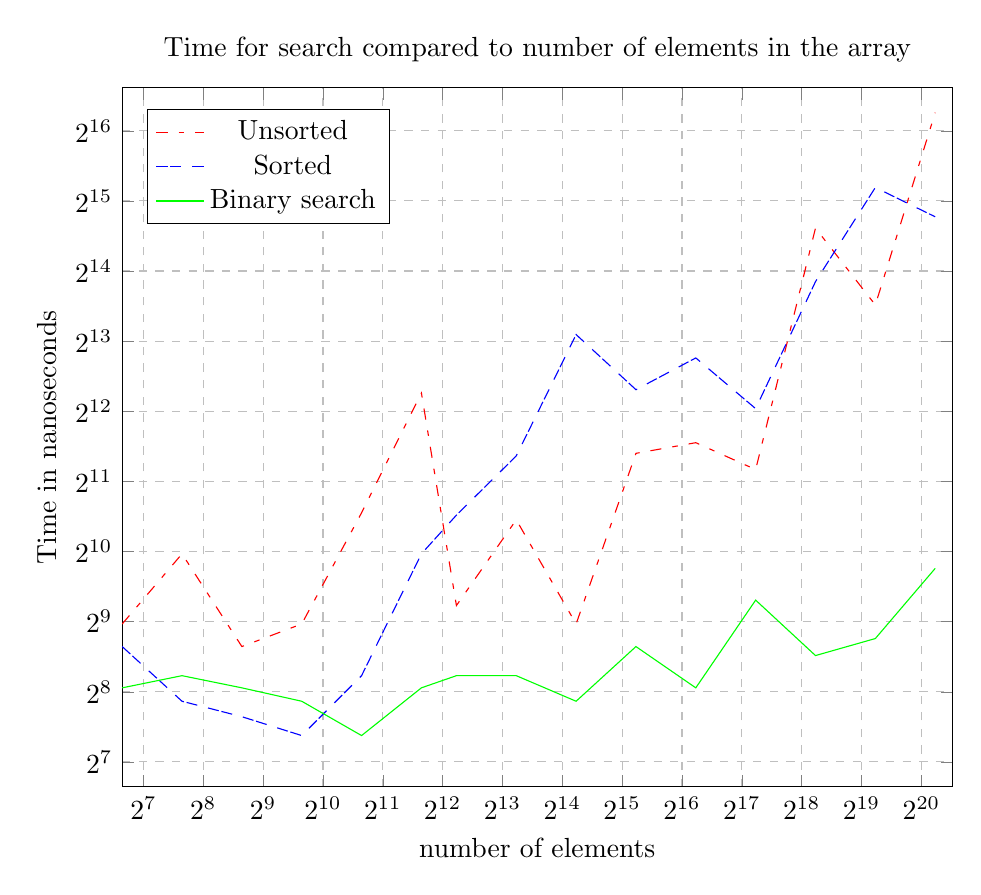
\begin{tikzpicture}
        \begin{axis}[
            title={Time for search compared to number of elements in the array},
            width=\linewidth,
            xlabel={number of elements},
            ylabel={Time in nanoseconds},
            xmode=log,
            log basis x={2},
            ymode=log,
            log basis y={2},
            xmin=100, xmax=1500000,
            ymin=100, ymax=100000,
            ymajorgrids=true,
            xmajorgrids=true,
            grid style=dashed,
            legend pos=north west,
        ]
        
        \addplot[
            color=red,
            dash pattern=on 4pt off 4pt on 2pt off 4pt,
            ]
            coordinates {
            (100,500)(200,1000)(400,400)(800,500)(1600,1500)(3200,4900)(4800,600)(9600,1400)(19200,500)(38400,2700)(76800,3000)(153600,2300)(307200,25000)(614400,11700)(1228800,78300)
            };
            \addlegendentry{Unsorted}
        \addplot[
            color=blue,
            dash pattern=on 4pt off 1pt on 4pt off 4pt,
            ]
            coordinates {
            (100,400)(200,233)(400,200)(800,166)(1600,300)(3200,1000)(4800,1466)(9600,2633)(19200,8733)(38400,5066)(76800,6933)(153600,4200)(307200,14733)(614400,37366)(1228800,27966)
            };
            \addlegendentry{Sorted}
        \addplot[
            color=green,
            ]
            coordinates {
            (100,266)(200,300)(400,266)(800,233)(1600,166)(3200,266)(4800,300)(9600,300)(19200,233)(38400,400)(76800,266)(153600,633)(307200,366)(614400,433)(1228800,866)
            };
            \addlegendentry{Binary search}
        
            
            
        \end{axis}
        \end{tikzpicture}
    \caption{Using binary search(samples are average of 3 measurements)}
    \label{fig:plot3}
\end{figure}

This now shows us how much more efficient this algorithm is as compared the the simple traversal of elements. From this graph we can generally equate the time complexity as logarithmic i.e. {\tt O(log(n))}. Knowing this we can estimate that an array with 64M elements would only take a comparatively small amount of additional time then 1M elements.

\section*{Recursive Binary Search}

When we’re at it, we might as well introduce an alternative way of implementing the binary search procedure. We will define a procedure recursive()
that will do a binary search in an array from a minimum index to a maximum index. The maximum index has to be at least as large as the minimum
index. We could for example search for a key between index 10 and 30 but
instead of just modifying our existing implementation we will do a trick; we
will call the method recursively.

\begin{minted}[
frame=single,
framesep=2mm,
baselinestretch=1.2,
fontsize=\footnotesize,
]{java}
    (...)
     private static boolean recursive(int[] arr, int key, 
        int min, int max) {
        
        int mid = min + ((max - min) / 2);
        if (arr[mid] == key) {
            return true;
        }
        if ((arr[mid] > key) && (min < mid)) {
            return recursive(arr, key, min, mid);
        }
        if ((arr[mid] < key) && (mid < max)) {
            return recursive(arr, key, mid + 1, max);
        }
        return false;
    }
    (...)
\end{minted}

In order for this recursive method to be interchangeable with the {\tt binary\textunderscore search} method I encapsulate it in a wrapper function which takes only the two parameters of the array and key and passes the additional two to the recursive function.

\begin{minted}[
frame=single,
framesep=2mm,
baselinestretch=1.2,
fontsize=\footnotesize,
]{java}
    (...)
    public static boolean recursive_search(int[] array, int key) {
        return recursive(array, key, 0, array.length - 1);
    }
    (...)
\end{minted}

And now we can compare the performance of all the search implementations discussed in this report:

\begin{figure}[H]
    \centering
    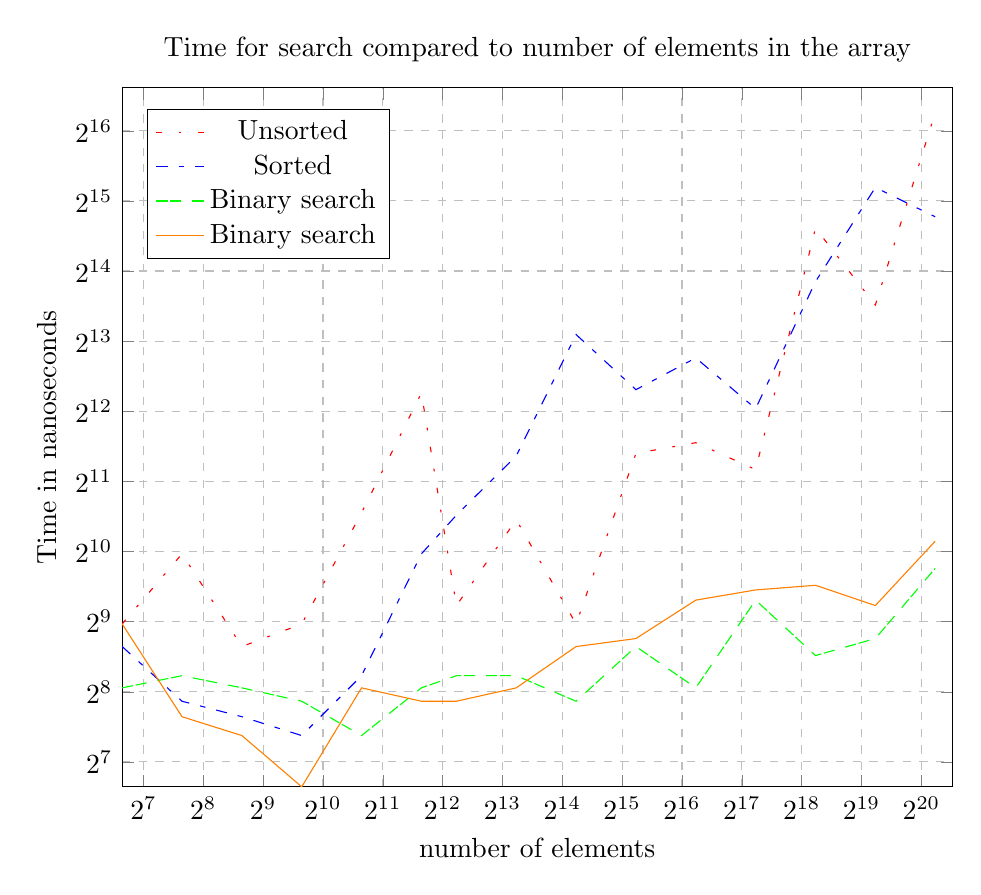
\begin{tikzpicture}
        \begin{axis}[
            title={Time for search compared to number of elements in the array},
            width=\linewidth,
            xlabel={number of elements},
            ylabel={Time in nanoseconds},
            xmode=log,
            log basis x={2},
            ymode=log,
            log basis y={2},
            xmin=100, xmax=1500000,
            ymin=100, ymax=100000,
            ymajorgrids=true,
            xmajorgrids=true,
            grid style=dashed,
            legend pos=north west,
        ]
        
        \addplot[
            color=red,
            dash pattern=on 2pt off 6pt on 1pt off 6pt,
            ]
            coordinates {
            (100,500)(200,1000)(400,400)(800,500)(1600,1500)(3200,4900)(4800,600)(9600,1400)(19200,500)(38400,2700)(76800,3000)(153600,2300)(307200,25000)(614400,11700)(1228800,78300)
            };
            \addlegendentry{Unsorted}
        \addplot[
            color=blue,
            dash pattern=on 4pt off 4pt on 2pt off 4pt,
            ]
            coordinates {
            (100,400)(200,233)(400,200)(800,166)(1600,300)(3200,1000)(4800,1466)(9600,2633)(19200,8733)(38400,5066)(76800,6933)(153600,4200)(307200,14733)(614400,37366)(1228800,27966)
            };
            \addlegendentry{Sorted}
        \addplot[
            color=green,
            dash pattern=on 4pt off 1pt on 4pt off 4pt,
            ]
            coordinates {
            (100,266)(200,300)(400,266)(800,233)(1600,166)(3200,266)(4800,300)(9600,300)(19200,233)(38400,400)(76800,266)(153600,633)(307200,366)(614400,433)(1228800,866)
            };
            \addlegendentry{Binary search}
        
         \addplot[
            color=orange,
            ]
            coordinates {
            (100,500)(200,200)(400,166)(800,100)(1600,266)(3200,233)(4800,233)(9600,266)(19200,400)(38400,433)(76800,633)(153600,700)(307200,733)(614400,600)(1228800,1133)
            };
            \addlegendentry{Binary search}   
            
        \end{axis}
        \end{tikzpicture}
    \caption{Recursive binary search(samples are average of 3 measurements)}
    \label{fig:plot4}
\end{figure}

Contrary to what I would think the recursive implementation does not deviate as much from the iterative binary search. We can be sure, though, that this tendency would not follow for larger array sizes.

\end{document}